\documentclass[letterpaper,12pt,oneside]{scrbook}


\usepackage[utf8]{inputenc}

\usepackage[spanish,es-nodecimaldot,es-tabla]{babel}

\usepackage{graphicx}

\usepackage{natbib}  % Usando paquete para citas

\usepackage{amsmath} % Notación

\usepackage{amssymb}

\usepackage{amsthm}  % Definiciones

\usepackage{longtable}

\usepackage{todonotes}   % insert [disable] to disable all notes

\usepackage[T1]{fontenc} % Required for accented characters

\usepackage{outlines}


\newcommand{\note}[4][]{\todo[author=#2,color=#3,size=\scriptsize,fancyline,caption={},#1]{#4}} % default


%For comments in a bubble on the document margins:

\newcommand{\ximena}[2][]{\note[#1]{Ximena}{green!40}{#2}}

\newcommand{\vic}[2][]{\note[#1]{Vic}{orange!40}{#2}}

\newcommand{\diego}[2][]{\note[#1]{Diego}{blue!40}{#2}}


%For inline comments:

\newcommand{\Ximena}[2][]{\ximena[inline,#1]{#2}\noindent}

\newcommand{\Vic}[2][]{\vic[inline,#1]{#2}\noindent}

\newcommand{\Diego}[2][]{\diego[inline,#1]{#2}\noindent}


% For code formatting

\def\code#1{\texttt{#1}}


% Teoremas y ejemplos

\theoremstyle{definition}

\newtheorem{exmp}{Ejemplo}[section]

\newtheorem{definition}{Definición}


\graphicspath{{./img/}}


\begin{document}

	\bibliographystyle{acl_natbib}  % Cargando estilo de bibliografia

	
	\author{Diego Alberto Barriga Martínez}

	\title{Etiquetador automático de la morfología del otomí usando predicción estructurada}

	\tableofcontents

	\maketitle

	
	% TODO: Pasar todo lo del protocolo aquí

	% Utilzar el tiempo pasado 

	
	\chapter{Introducción}

	
	% Capitulo corto con el objetivo, hipótesis y tocar los temas del marco teorico de forma muy superficial. Se definen en el marco teorico

	
	\section{Lengua otomí}

	
	En esta sección se menciona los lugares donde se describe el idioma otomí de forma somera, se mencionan algunos lugares donde es hablado el otomí y características fundamentales de la lengua.

	
	\subsection{Origen}

	
	% Pie de pagina, no meter cosas tangenicales. Citar esta definicion

	La palabra otomí es de origen náhuatl (singular: \textit{otomitl}, plural: \textit{otomí}). Por otra parte, los otomíes se nombran a sí mismos \textit{ñähñu}\footnote{Existen organizaciones indígenas, como el Consejo de la Nacionalidad Otomí, que escriben la auto-denominación como hñätho hñähñu y también ñätho ñähño. Sin embargo, esta auto denominación puede variar.}, que significa "los que hablan otomí".

	
	Los grupos indígenas que hablan el idioma otomí se encuentran en diversas partes del territorio mexicano como: Estado de México, Querétaro, Hidalgo, Puebla y Veracruz \citep{barrientos2004otomies}. El otomí es una lengua indígena una gran variación dialectal que depende de su distribución geográfica.

	
	En el Estado de México el pueblo \textit{ñähñu} está disperso por varios municipios tales como: Toluca, Lerma, Chapa de Mota, Aculco, Amanalco, Atizapán de Zaragoza, por mencionar algunos. En otros municipios como Naucalpan, Ecatepec, Nezahualcóyotl y Tlalnepantla se pueden encontrar hablantes por efectos de la migración. Según \citet{barrientos2004otomies} la población total de hablantes otomíes en el Estado de México supera los cien mil, sin embargo, datos actuales .

	
	En concreto existen \textbf{nueve} variantes del otomí y cabe recalcar que dicha variación puede presentarse incluso dentro del mismo estado. Tan solo el Estado de México presenta tres variantes del otomí: El otomí de Tilapa, hablado en el municipio de Santiago Tianguistenco; el Otomí de Acazulco, del municipio de San Jerónimo Acazulco; y el Otomí de Toluca, de San Andrés Cuexcontitlán.

	
	\section{Problemática}

	
	% TODO: Cambiar las citas a bibtex

	El NLP es un área de la computación que permite reconocer, procesar e interpretar el lenguaje humano dentro de un sistema computacional. El objetivo de esta área es hacer que las computadoras realicen tareas que involucran el lenguaje humano. Algunas tareas generales consisten en permitir la comunicación humano-máquina, o simplemente hacer un exitoso procesamiento de texto o voz humanos \citep{jurafsky2008speech}. Ejemplos de aplicación actuales son los traductores automáticos, asistentes personales que reconocen voz, motores de búsquedas en Internet, análisis de sentimientos en textos,  síntesis de voz, etiquetado de textos y muchas más aplicaciones.

	
	% Voy de lo mas general a lo particular

	Una de las tareas más populares de NLP es el etiquetado automático de textos. Este etiquetado puede realizarse a diferentes niveles lingüísticos, por ejemplo, morfosintáctico (\textit{Part Of Speech tagging, POS}), sintáctico (\textit{parsing}), morfológico, etc.  El nivel morfológico tiene que ver con la estructura interna de las palabras \citep{haspelmath2013understanding}; en particular, existe un tipo de etiquetado, de gran importancia para el análisis lingüístico, llamado glosado que asigna etiquetas a las unidades que conforman a una palabra. 

	
	% Hablando de ML

	Para lograr lo anterior, los enfoques actuales aplican técnicas de ML. El ML es un subcampo de la Inteligencia Artificial (IA), que constituye un enfoque de resolución de problemas caracterizado por estimar una solución a partir de la experiencia \citep{mitchell1997machine}.  La experiencia se refiere a datos etiquetados (ejemplos) que permiten inferir un modelo estadístico de aprendizaje. Entre los métodos de ML ampliamente utilizados se pueden mencionar las Support Vector Machines (SVMs), árboles de decisión, o bien los modelos gráficos, como las redes neuronales o los métodos generativos, solo por mencionar algunos. Para las tareas de etiquetado en NLP generalmente se utilizan modelos gráficos supervisados, por ejemplo, modelos ocultos de Markov (\textit{Hidden Markov Models, HMM}).

	
	% Introduccion de la problematica

	No obstante, el lenguaje natural es complejo y dinámico, ya que tiene fenómenos que hacen que las tareas de reconocimiento, generación y procesamiento se vuelvan difíciles para las computadoras. Adicionalmente, existen escenarios donde estos métodos no son efectivos como es el caso de las lenguas de bajos recursos, que son lenguas que tienen pocos recursos digitales con los que trabajar. Por ejemplo, si se tienen pocos datos iniciales para el entrenamiento del modelo de aprendizaje las predicciones serán poco precisas o equivocadas. Los bajos recursos son un escenario común en México donde, a pesar de que existe una rica diversidad lingüística, gran parte de las lenguas originarias no poseen contenido web ni publicaciones digitales y por tanto carecen también de tecnologías del lenguaje.  El escenario mencionado anteriormente supone un reto para los métodos de aprendizaje convencionales, que requieren de grandes cantidades de datos de entrenamiento para funcionar correctamente. Por lo tanto, es un importante reto de investigación desarrollar aproximaciones que funcionen con lenguas de escasos recursos. En particular, en este trabajo nos enfocamos en el glosado automático del otomí, una lengua con gran riqueza morfológica y con escasez de recursos digitales.

	
	El glosado puede ser un primer paso para el desarrollo de más tecnologías del lenguaje; no solo para el otomí, que presenta un grado de extinción acelerada \Diego{¿Esta cita donde la puedo encontrar?} \Vic{Se refiere a la información de la Comisión nacional para el Desarrollo de pueblos Indígenas, pero ahora es el IMPI https://www.gob.mx/inpi} (CDI), sino para las 68 agrupaciones lingüísticas que se hablan en México.

	
	\section{Objetivo}

	
	Diseñar e implementar un etiquetador morfológico para el otomí basado en técnicas de Procesamiento del Lenguaje Natural (\textit{Natural Language Processing, NLP}) con Aprendizaje de Máquina (\textit{Machine Learning, ML}). En particular, se hará énfasis en métodos de aprendizaje estructurado débilmente supervisados. Específicamente, se aplicará \textit{Conditional Random Fields (CRF)} para etiquetado morfológico (glosado) del otomí, una lengua de bajos recursos.

	
	\section{Hipótesis}

	
	Se espera obtener un modelo que produzca glosa para el otomí, generada automáticamente, con base en el entrenamiento con pocos ejemplos previamente etiquetados. Al obtener una buena exactitud en la predicción automática de glosa se apoyaría a los anotadores humanos a reducir trabajo repetitivo y exhaustivo. Además, se espera obtener avances de una metodología adaptable a un mayor número de lenguas mexicanas. Sería deseable que esta metodología experimental pueda ser replícale en otras lenguas habladas en México.

	
	\chapter{Avances en etiquetadores automáticos}

	
	% Mencionar los bajos recursos

	
	\section{Marco teórico}\label{sec:marco}

	
	% Se tiene que explicar los conceptos de low resouces 

	
	% .Etiquetadores a diferentes niveles lingüísticos

	% &Etiquetadores a nivel morfológico

	% &modelos gráficos

	% Que es un etiquetador

	% Bio Labels

	% Que es la morfología 

	% que es la glosa

	% Low resources

	% Algoritmo L&BFGS

	% L1 & L2

	
	% &NLP

	\subsection{Natural Language Processing (NLP)}

	% Introduccion

	
	\subsection{Etiquetadores}

	
	% &Machine learning

	\subsection{Machine Learning (ML)}

	
	\subsection{Modelos gráficos}

	
	% Los límites de los modelos gráficos para bajos recursos

	
	% Cierre de los modelos graficos y comenzar a hablar de CRF

	% No perder de vista que los CRFs son modelos graficos pero con ventajas

	
	\subsubsection{Los límites de los modelos gráficos en para bajos recursos}

	
	En este capítulo se explicará qué ventajas tienen los \emph{Conditional Random Fields (CRF)} sobre otros modelos de aprendizaje, se mencionan formalmente los elementos fundamentales que describen los \emph{CRF's}.

	
	En lingüística computacional una tarea de interés es el procesamiento estadístico del lenguaje natural, en particular, el etiquetado y segmentación de secuencias de datos. En ese sentido, es habitual la utilización de \textbf{modelos generativos}, cómo los \textit{Hidden Markov Models (HMMs)}, o \textbf{modelos condicionales}, como los \textit{Maximum Entropy Markov Models (MEMMs)}.

	
	Por una parte, los modelos generativos intentan modelar una probabilidad conjunta $P(x,y)$ sobre observaciones y etiquetas. Para definir esta probabilidad conjunta se necesita enumerar todas las observaciones posibles. Las limitantes de este enfoque son de diversas índoles como las grandes dimensionalidades en el vector de entrada $X$, la dificultad de representar múltiples características que interactúan unas con otras y dependencias complejas que hacen la construcción de la distribución de probabilidad un problema intratable con un enfoque computacional.

	
	Por otro lado, una solución a las limitantes de los modelos generativos es un modelo condicional. Estos modelos no son tan estrictos como los primeros al momento de asumir independencias en las observaciones. Los modelos condicionales especifican la probabilidad de posibles etiquetas dada una secuencia de observación.

	
	Consecuencia de lo anterior, no se gasta esfuerzo en modelar las observaciones, dado que en al momento de realizar pruebas estas observaciones son fijas. Segundo, la probabilidad condicional puede depender de características arbitrarias y no dependientes de la secuencia de observación sin forzar al modelo a tomar en cuenta la distribución de estas características, permitiendo que el modelo sea tratable \citep{lafferty2001conditional}.

	
	Un ejemplo de estas ventajas con los \textit{MEMMs} que son modelos secuenciales de probabilidad condicional. Sin embargo, estos modelos y otros que son no generativos, de estados finitos y que son clasificadores basados en el estado siguiente comparten una debilidad llamada \emph{label bias problem}. \citet{lafferty2001conditional} define que existe el \emph{label bias problem} cuando "las transiciones que dejan un estado compiten solo entre sí, en lugar de entre todas las demás transiciones en el modelo".

	
	Dado que las transiciones son las probabilidades condicionales de los siguientes posibles estados una observación puede afectar cuál será el estado siguiente sin tomar en cuenta que tan adecuado será este. Por tanto, se tendrá un sesgo en los estados con menos transiciones de salida.

	
	\subsection{Conditional Random Fields}

	
	Como menciona \citet{sutton2012introduction} modelar las dependencias entre las entrada puede conducir a modelos intratables, pero ignorar estas dependencias puede reducir el rendimiento.

	
	Dado el que problema abordado en este trabajo, dónde se requiere del etiquetado de secuencias y es en contexto de bajos recursos lingüísticos, se hace necesario utilizar un enfoque más conveniente.

	
	Los \textit{Conditional Random Fields (CRFs)} son un framework para la creación de modelos probabilístico utilizado en técnicas de aprendizaje estructurado. Tienen las ventajas de los \textit{MEMMs} y, en principio, solucionan el \emph{label bias problem}. El framework tiene un solo modelo exponencial para la probabilidad conjunta de todas las secuencias de las etiquetas de salida dada la secuencia de observación. En contraste los \emph{MEMMs} usan modelos exponenciales para cada probabilidad condicional de los estados siguientes dado el estado actual.

	
	Formalmente \citet{lafferty2001conditional} definen los \textit{CRFs} como a continuacion se enuncia:

	
	\begin{definition}

		Sea $G = (V,E)$ una gráfica tal que $\mathbf{Y} = (\mathbf{Y}_{v})_{v \in V}$, entonces esa $\mathbf{Y}$ es indexada por los vertices de $G$. Entonces $(\mathbf{X}, \mathbf{Y})$ es un \textsf{conditional random field} en caso de que las variables aleatorias $\mathbf{Y}$ se condicionen por $\mathbf{X}$, la variable aleatoria $\mathbf{Y}_{v}$ cumple la \textit{propiedad de Markov} con respecto a la gráfica: $p(\mathbf{Y}_{v}|\mathbf{X},\mathbf{Y}_{w},w \ne v) = p(\mathbf{Y}_{v}|\mathbf{X},\mathbf{Y}_{w},w \sim v)$, dónde $w \sim v$ significa que $w$ y $v$ son vecinos en $G$.

	\end{definition}

	
	En esta tesis, para el modelado de secuencias, se utiliza la forma más sencilla de la gráfica $G$ dónde es una cadena simple o línea. Esto quiere decir que $G = (V = \{1,2,...m\}, E = \{(i,i+1)\})$. A este tipo de \textit{CRFs} se les conoce como \textit{linear-chain CRFs}. Como menciona \citet{lafferty2001conditional} "si la gráfica $G = (V,E)$ de $\mathbf{Y}$ es un árbol (del cual una cadena es el ejemplo más sencillo), los \textit{cliques} son los límites y vertices. Entonces, por el teorema de los \textit{random fields} \citep{hammersley1971markov}, la distribución conjunta sobre las etiquetas de secuencias $\mathbf{Y}$ y $\mathbf{X}$ tiene la forma:

	
	% TODO: Poner tag

	% TODO: Explicar esta ecuacion sobre que es son las lambdas, porque hay dos sumandos, porque el símbolo de proporcionalidad, 

	\begin{equation}

	p{_{\theta}}(y|x) \propto \exp \bigg( \sum\limits_{e \in \mathbf{E},k} \lambda_{k}f_{k}(e,\mathbf{y}|_{e},\mathbf{x}) + \sum\limits_{v \in \mathbf{V},k}\mu_{k}g_{k}(v,\mathbf{y}|_{v},\mathbf{x}) \bigg)

	\end{equation}

	
	% TODO: Mencionar la ecucacion

	% TODO: Descripcion de la estimacion de parametros y característica de la función de perdida

	
	De la ecuación  se destacan $f_{k}$ y $g_{k}$ que representan las \textit{feature functions}. Estas están definidas y son fijas. Las \textit{feature functions} de está tesis serán descritas más adelante. 

	
	\section{Estado del arte}

	
	Los \textit{CRFs} han sido utilizados para la clasificación de regiones en una imagen, estimar el puntaje en un juego de Go, segmentar genes en una hebra de ADN y análisis sintáctico de lenguaje natural en un texto por mencionar algunas \citep{sutton2012introduction}.

	
	
	\subsection{Trabajos sobre bajos recursos}

	% Hablar del trabajo para Lezgi

	Con base en el trabajo previo de \citep{moeller2018automatic} donde se utilizan técnicas de NLP y ML para tratar para el idioma Lezgi se plantea como hipótesis que dado el tamaño del corpus y la glosa que contiene 

	se obtendrá texto correctamente glosado con una precisión de al menos 80\%.

	
	% Papers que hablen del tema de etiquetado automático 2010 para acá

	
	% Redes neuronales,

	% Mencion de trabajo y papers actuales hacen algo similar

	
	
	\chapter{Etiquetador morfológico para el otomí (Metodología)}

	
	En este capitulo se describe el corpus utilizado en este trabajo, se mostrará la arquitectura propuesta para la generación automática de glosa para el idioma otomí. Adicionalmente, se explicará el diseño e implementación del \textit{pipeline} que incluye, entre otras cosas, la determinación de las \textit{feature functions}.

	
	%TODO: Descripción de la estimacion de parametros y caracteristica de la funcion de perdida

	Los \textit{CRFs} muestran claras ventajas sobre otros métodos de aprendizaje basados en gráficas. Su habilidad de tomar las virtudes de los modelos generativos y de los modelos condicionales presentan a este \textit{framework} como una opción para el contexto de los bajos recursos digitales que nos impone, como se describirá más adelante, el tamaño del corpus. En ese sentido, los \textit{CRFs} se utilizaron para predecir secuencias de etiquetas, utilizando el enfoque del aprendizaje estructurado, que describen las unidades morfológicas dentro de una palabra, de una variante en particular del otomí. 

	
	% Particularidades del corpus (Análisis cualitativo y cuantitativo)

	\section{Corpus: otomí de Toluca}

	
	% Siempre ir de lo general a lo particular

	
	% Tipo de otomi y características de la variante

	La clasificación lingüística introduce al otomí dentro de las lenguas otomianas, las cuales a su vez pertenecen a la rama otopame de la familia otomangue \citep{barrientos2004otomies}. Cada variante muestra particularidades fonológicas, morfológicas, sintácticas y léxicas. En el tratamiento de textos por medio de técnicas de \textit{NLP} se requiere que estos textos estén normalizados y homogéneos. Lo anterior propicia la obtención del mejor desempeño posible en los diversos métodos de aprendizaje automático. Mas adelante se describirá el proceso de preprocesamiento aplicado al corpus.

	
	% Otomi en general, Familia y rama

	Se utilizó un corpus en otomí que, además, cumple la característica de estar glosado. Se trabajó con la variante del otomí de Toluca de la región de San Andrés Cuexcontitlan.

	
	% De donde vienen los textos, quien lo glosa y quien lo recolecta

	Esta tesis recogió un corpus basado en el trabajo de \citet{lastra1992otomi} titulado \emph{El otomí de Toluca} y que a su vez fue etiquetado y glosado manualmente por el lingüista Víctor Germán Mijangos de la Cruz\footnote{TODO: Liga del repo}. Este corpus es un subconjunto del corpus paralelo español-otomi que se encuentra en la plataforma web Tsunkua\footnote{https://tsunkua.elotl.mx/}. Además, se agregaron 81 lineas de casos poco usuales y que son fenómenos poco frecuentes y por tanto particularmente difíciles de predecir. El subconjunto del corpus utilizado en la sección experimental está descrito en la tabla \ref{table:corpus_length:1}, donde se encuentra el tamaño de las etiquetas POS y el tamaño de la glosa y en la tabla \ref{table:corpus_text:1}, donde se puede ver los tipos de textos presentes en el corpus.

	
	% Tokens y tipos de Palabras

	
	% Numero de etiquetas diferentes

	\begin{table}

		\centering

		\begin{tabular}{c | c}

			\textbf{Categoría} & \textbf{Cuenta} \\ \hline

			Tokens (POS) & 8578\\

			Tipos (POS) & 44\\

			Tokens (Glosa) & 14477\\

			Tipos (Glosa) & 112\\

			\textbf{Total de oraciones etiquetadas} & 1786 \\ 

		\end{tabular}

		\caption{Tamaño del corpus}

		\label{table:corpus_length:1}

	\end{table}

	
	\begin{table}

		\centering

		\begin{tabular}{ c | c }

			\textbf{Textos} & \textbf{Número} \\ \hline

			Narrativos & 32 \\

			Dialogados & 4  \\

			\textbf{Total de textos}  & 36 \\

		\end{tabular}

		\caption{Textos del corpus}

		\label{table:corpus_text:1}

	\end{table}

	
	Los textos que componen el corpus fueron construidos a partir de las aportaciones de diez hablantes distintos de entre diez y setenta y tres años, de los cuales, siete son de sexo femenino y tres masculino \citep{lastra1992otomi}. 

	
	% TODO: Características esenciales que tiene que ver con el etiquetado POS de las lenguas otomies

	% TODO: Descripción detalla del etiquetado POS

	
	% Reorganizar esto

	% Seccion sin seccion de POS, glosa, Bio labels sin tablas

	% Citar el estándar de etiquetas https://www.eva.mpg.de/lingua/pdf/Glossing&Rules.pdf

	
	% Mencionar que hay etiquetas en si mismas pero quitarlas de la tabla

	Los tipos de etiquetas \textit{POS} presentes en el corpus se pueden observar en la tabla \ref{table:pos_types}. Dentro del conjunto de estas las etiquetas encontramos un subconjunto con elementos como \textsf{buena.vista}, \textsf{nada.más} y \textsf{zapata}. Estos ejemplos son una forma de glosa muy común en el uso lingüístico y no están incluidos en la tabla \ref{table:pos_types} pues son descriptivos en sí mismos. Presentamos una descripción de las etiquetas en la tabla \ref{table:pos_descr}. \Vic{Esta forma de glosar es común en el uso lingüístico, no vale la pena presentarlo en la tabla pues son descriptivos por sí mismos.}

	
	\begin{table}

		\centering

		\begin{tabular}{| c | c | c | c | c |}

			\hline

			v & obl & det & cnj & dem \\ 

			unkwn & n & neg & p.loc & prt \\

			conj.adv & dim & gen & cond & it \\

			lim & aff & loc & dec & conj  \\

			cord & san & cnj.adv & regular/v & adv \\

			adj & & & & \\

			\hline

		\end{tabular}

		\caption{Tipos de etiquetas \textit{POS}} 

		\label{table:pos_types}

	\end{table}

	

	\begin{table}

		\centering

		\begin{tabular}{ c  c | c  c}

			\textbf{Etiqueta} & \textbf{Significado} & \textbf{Etiqueta} & \textbf{Significado} \\ \hline

			v & verbo & obl & oblicuo \\

			det & determinante & cnj & conjunción \\

			dem & demostrativo & unkwn & desconocido\\ 

			n & sustantivo & neg & negativo \\

			p.loc & partícula locativoa & prt & partícula \\

			conj.adv & conjunción adversativa & dim & diminutivo \\

			gen & genitivo & cond & condicional\\

			it & iterativo & lim & limitativo \\ 

			aff & afirmativo & loc & locativo \\

			dec & decimal & conj & conjunción \\

			cord & coordinación & cnj.adv & conjunción adversativa \\

			regular/v & verbo regular & & \\

		\end{tabular}

		\caption{Descripción de etiquetas \textit{POS}}

		\label{table:pos_descr}

	\end{table}

	
	Para las etiquetas de Glosa nos basamos en las reglas de \citet{comrie2008leipzig} desarrolladas por el departamento de lingüística del Instituto Max Planck y el Departamento de lingüística de la Universidad de Leipzing. El estándar consiste en diez reglas para la sintaxis y la semántica de glosas interlineales. y un apéndice con un lexicón propuesto de etiquetas de categorías abreviadas \citep{comrie2008leipzig}. Si bien las reglas cubren parte de las necesidades lingüísticas en el glosado de textos, tambien, son flexibles y se pueden agregar o modificar las convenciones dependiendo de las necesidades.

	
	Los tipos de etiquetas de glosa presentes en el corpus se encuentran en la tabla \ref{table:gloss_types}. Los números al inicio de algunas etiquetas significan las personas gramaticales. Existen combinaciones de varias etiquetas que son separadas por puntos. Por ejemplo, \textsf{pl.exc} es una combinación de las etiquetas "plural" y "exclusivo". El significado para cada glosa se muestra en la tabla \ref{table:gloss_desc}. En esta tabla se omitieron las variaciones de etiquetas con personas gramaticales para compactarla.

	
	
	\begin{table}

		\centering

		\begin{tabular}{| c | c | c | c | c |}

			\hline

			stem & det & 3.cpl & psd & lim \\

			prag & 3.icp & lig & det.pl & 1.icp \\

			3.pot & ctrf & 1.pot & pl.exc & 1.cpl \\

			dem & 1.pss & dim & pl & 1.obj \\

			ila & 2.icp & 1.prf & 3.cnt & 3.obj \\

			loc & mod & 1.cnt & 3.pls & prt \\

			it & dual.exc & 3.prf & 3.icp.irr & 3.pss \\

			2.pss & 1.enf & med & dual & p.loc \\

			2.cnt & 2 & 3.imp & int & neg \\

			1.icp.irr & 1.cpl.irr & 2.obj & aum & 1.pls \\

			2.cpl & 2.prf & gen & com & 2.pot\\

			adj & cond  & 3.cpl.irr & 1.sg & encl \\

			3.sg & 3.pss.pl & spt & 1.irr & 2.enf \\

			conj.adv & caus & con & chico & eh \\

			comp & prf & dist mov & 3.irr & det.dem\\

			dcl & nom & 2.icp.irr & & \\

			\hline

		\end{tabular}

		\caption{Glosa}

		\label{table:gloss_types}

	\end{table}

	
	\Vic{También pongo la tabla para las glosas, pero la reduzco, los números 1,2 y 3 son las personas. Creo que se pueden quitar las etiquetas que se ya están en la tabla anterior. Tamboén hay que acomodar las tablas para que se vean mejor}

	
	\begin{table}

		\centering

		\begin{tabular}{ c  c | c  c }

			\textbf{Glosa} & \textbf{Significado} & \textbf{Glosa} & \textbf{Significado}\\\hline

			stem & base & ctrf & contrafactual \\

			cpl & completivo & dem & demostrativo \\

			icp & incompletivo & dim & diminutivo \\

			pot & potencial & ila & ilativo \\

			ctn & continuativo & mod & modo \\

			prf & perfecto & loc & locativo \\

			pls & pluscuamperfecto & prt & partícula \\

			irr & irrealis & it & iterativo \\

			imp & imperativo & enf & enfático \\

			psd & pasado & neg & negativo \\

			pl & plural & int & interrogativo \\

			sg & singular & aum & aumentativo \\

			ex & exclusivo & gen & genitivo \\

			pss & posesivo & com & comitativo \\

			obj & objeto & adj & adjetivo \\

			med & voz media & encl & enclítico \\

			dual & número dual & enf & enfático \\

			det & determinante & caus & causativo \\

			lim & limitativo & comp & comparativo \\

			lig & ligadura & dcl & declarativo \\

			prag & partícula pragmática & \\

		\end{tabular}

		\caption{Descripción de Glosa}

		\label{table:gloss_desc}

	\end{table}

	
	
	\subsection{Tokens}

	
	% TODO: Hablar de como el corpus es de bajos recursos

	
	
	\begin{table}[ht]

		\centering

		\begin{tabular}{c | c}

			\textbf{Etiqueta} & \textbf{Tokens} \\ \hline

			v & 2596 \\

			obl & 2447 \\

			det & 975 \\

			cnj & 837 \\

			dem & 543 \\

			unkwn & 419 \\

			n & 273 \\

			neg & 178 \\

			p.loc & 81 \\

			prt & 49 \\

		\end{tabular}

		\caption{POS (Primeros 10)}

		\label{table_pos_tokens}

	\end{table}

	
	
	\begin{table}[ht]

		\centering

		\begin{tabular}{c | c}                            

			\textbf{Etiqueta} & \textbf{Tokens} \\ \hline

			stem & 7527 \\

			det & 733 \\

			3.cpl & 450 \\

			psd & 418 \\

			lim & 374 \\

			prag & 362 \\

			3.icp & 346 \\

			lig & 289 \\

			det.pl & 271 \\

			1.icp & 270 \\

		\end{tabular}

		\caption{Glosa (Primeros 10)}

		\label{table_gloss_tokens}

	\end{table}

	
	
	% Grafica de Zipf para las etiquetas POS

	% Distribucion de etiquetas

	\subsection{Distribución de etiquetas}

	
	\begin{figure}[ht]

		\centering

		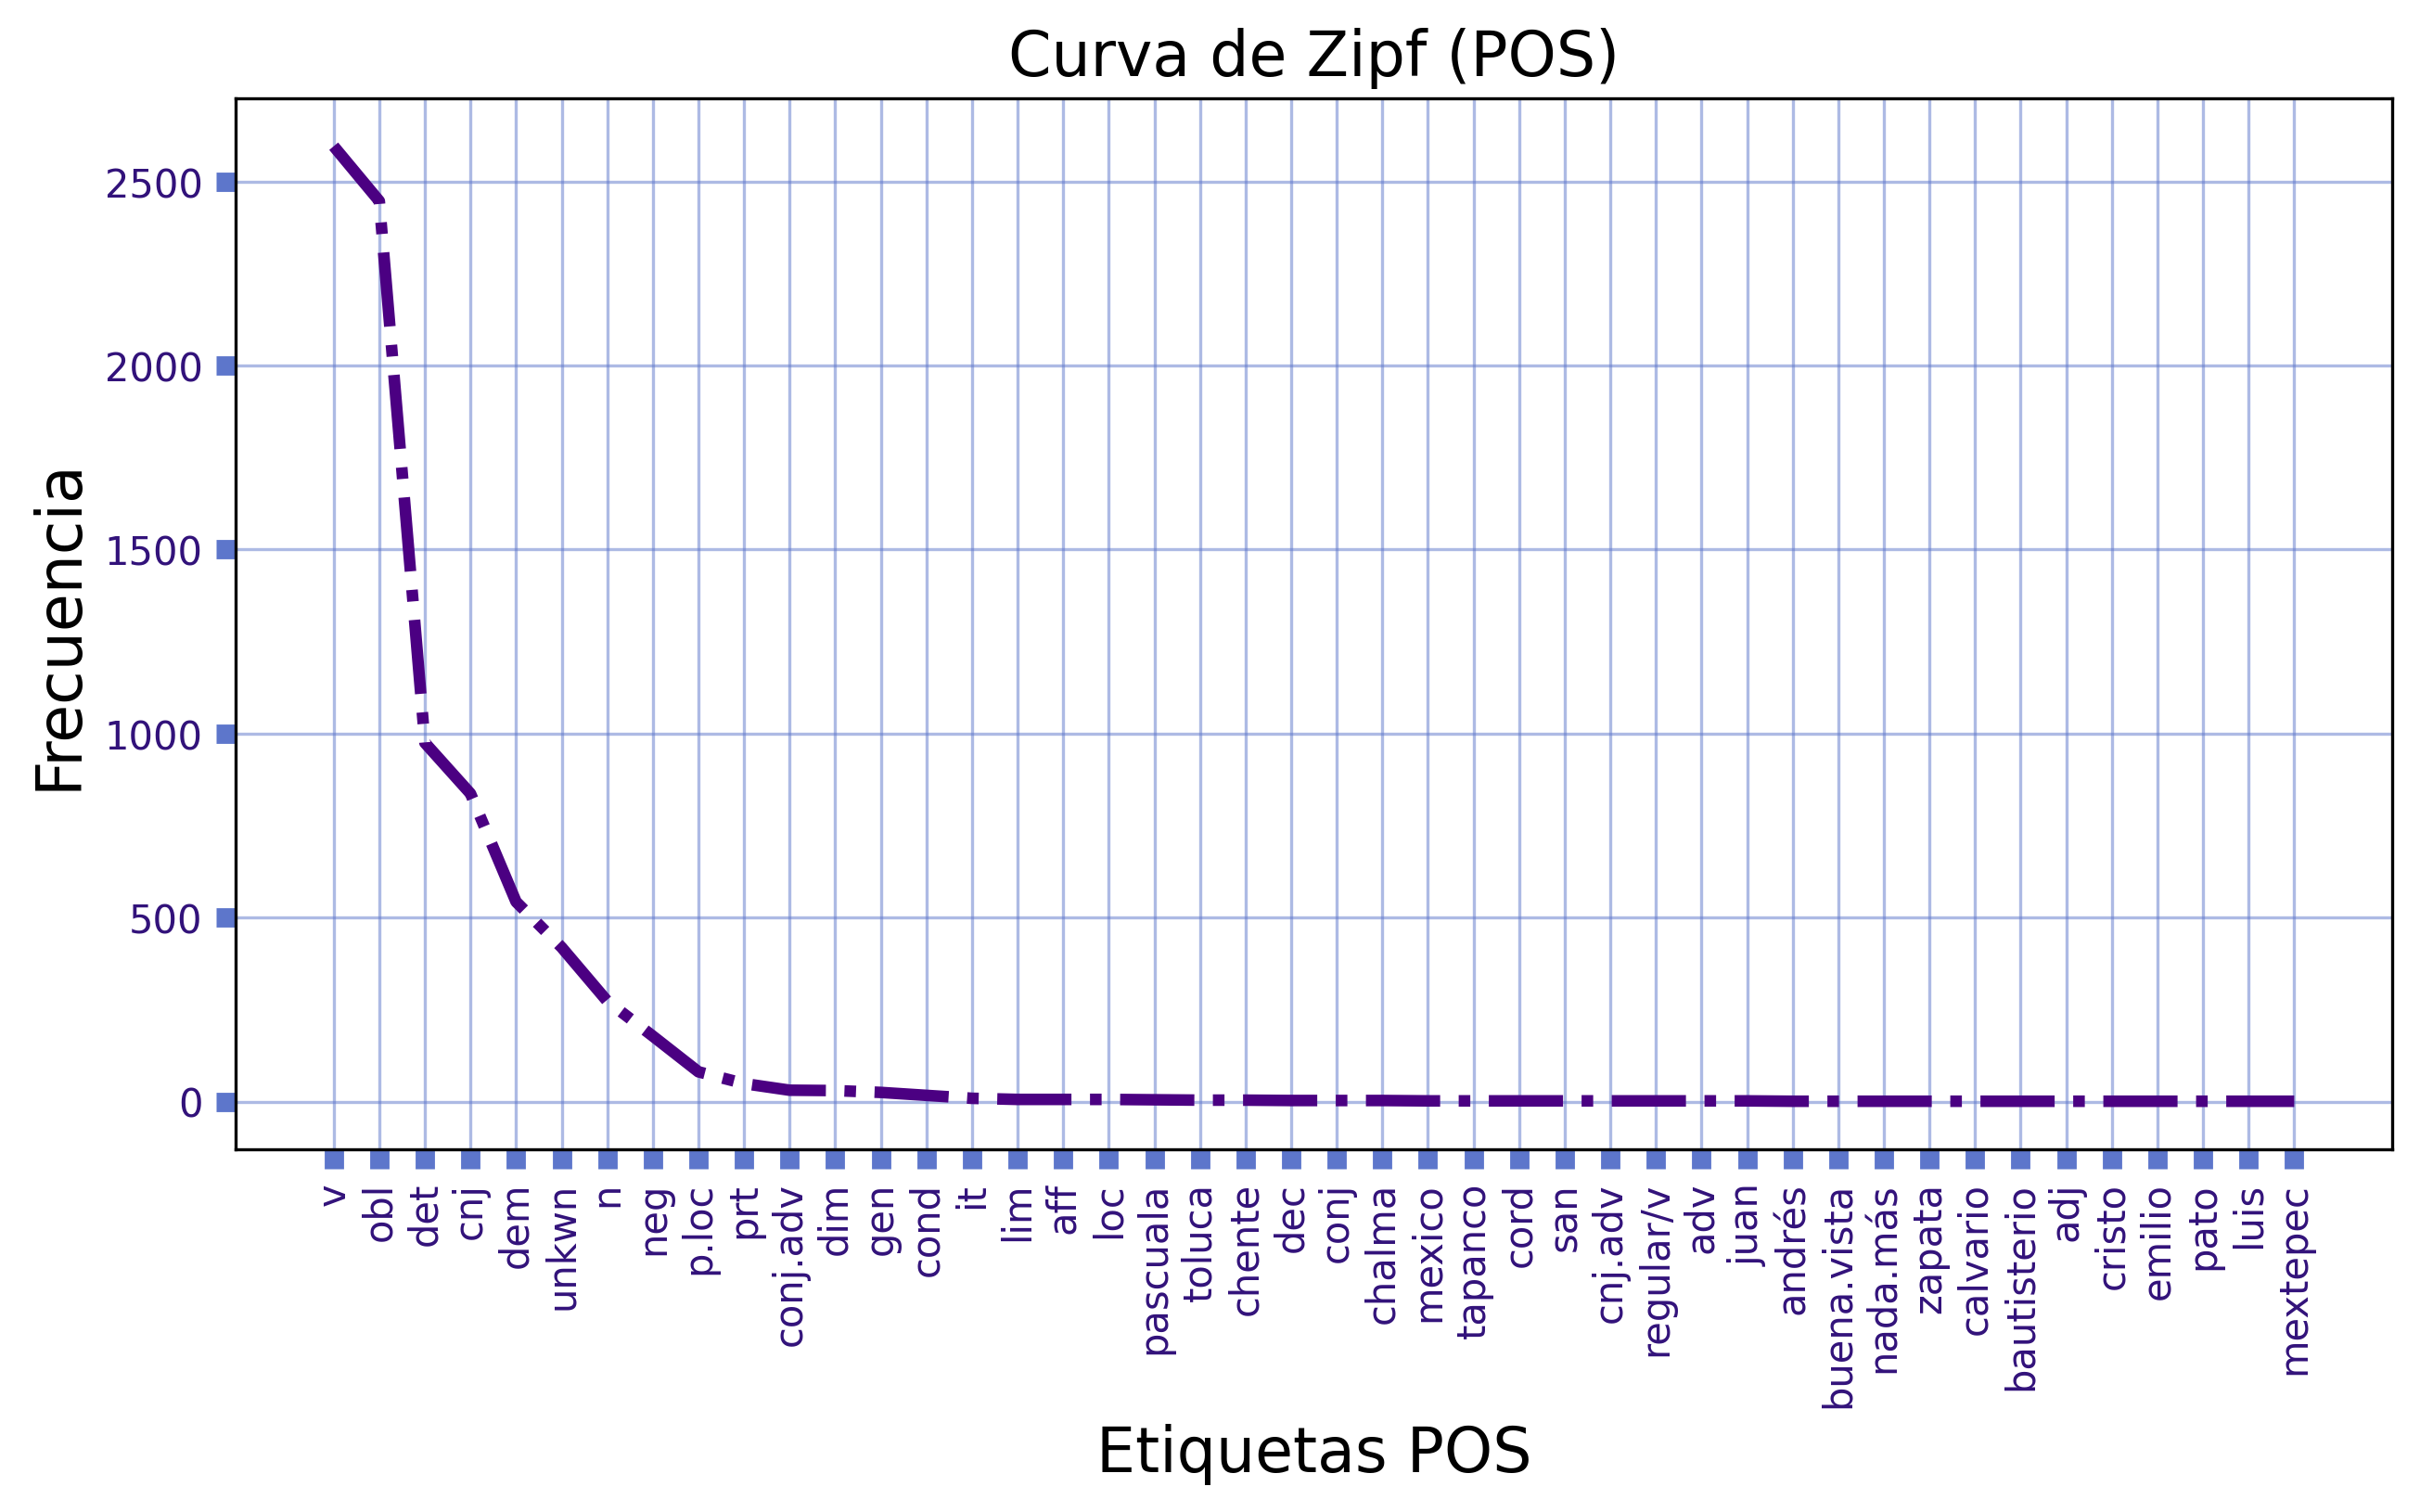
\includegraphics[width=\textwidth]{zipf_pos}

		\caption{Distribución de etiquetas POS}

	\end{figure}

	
	\begin{figure}[ht]

		\centering

		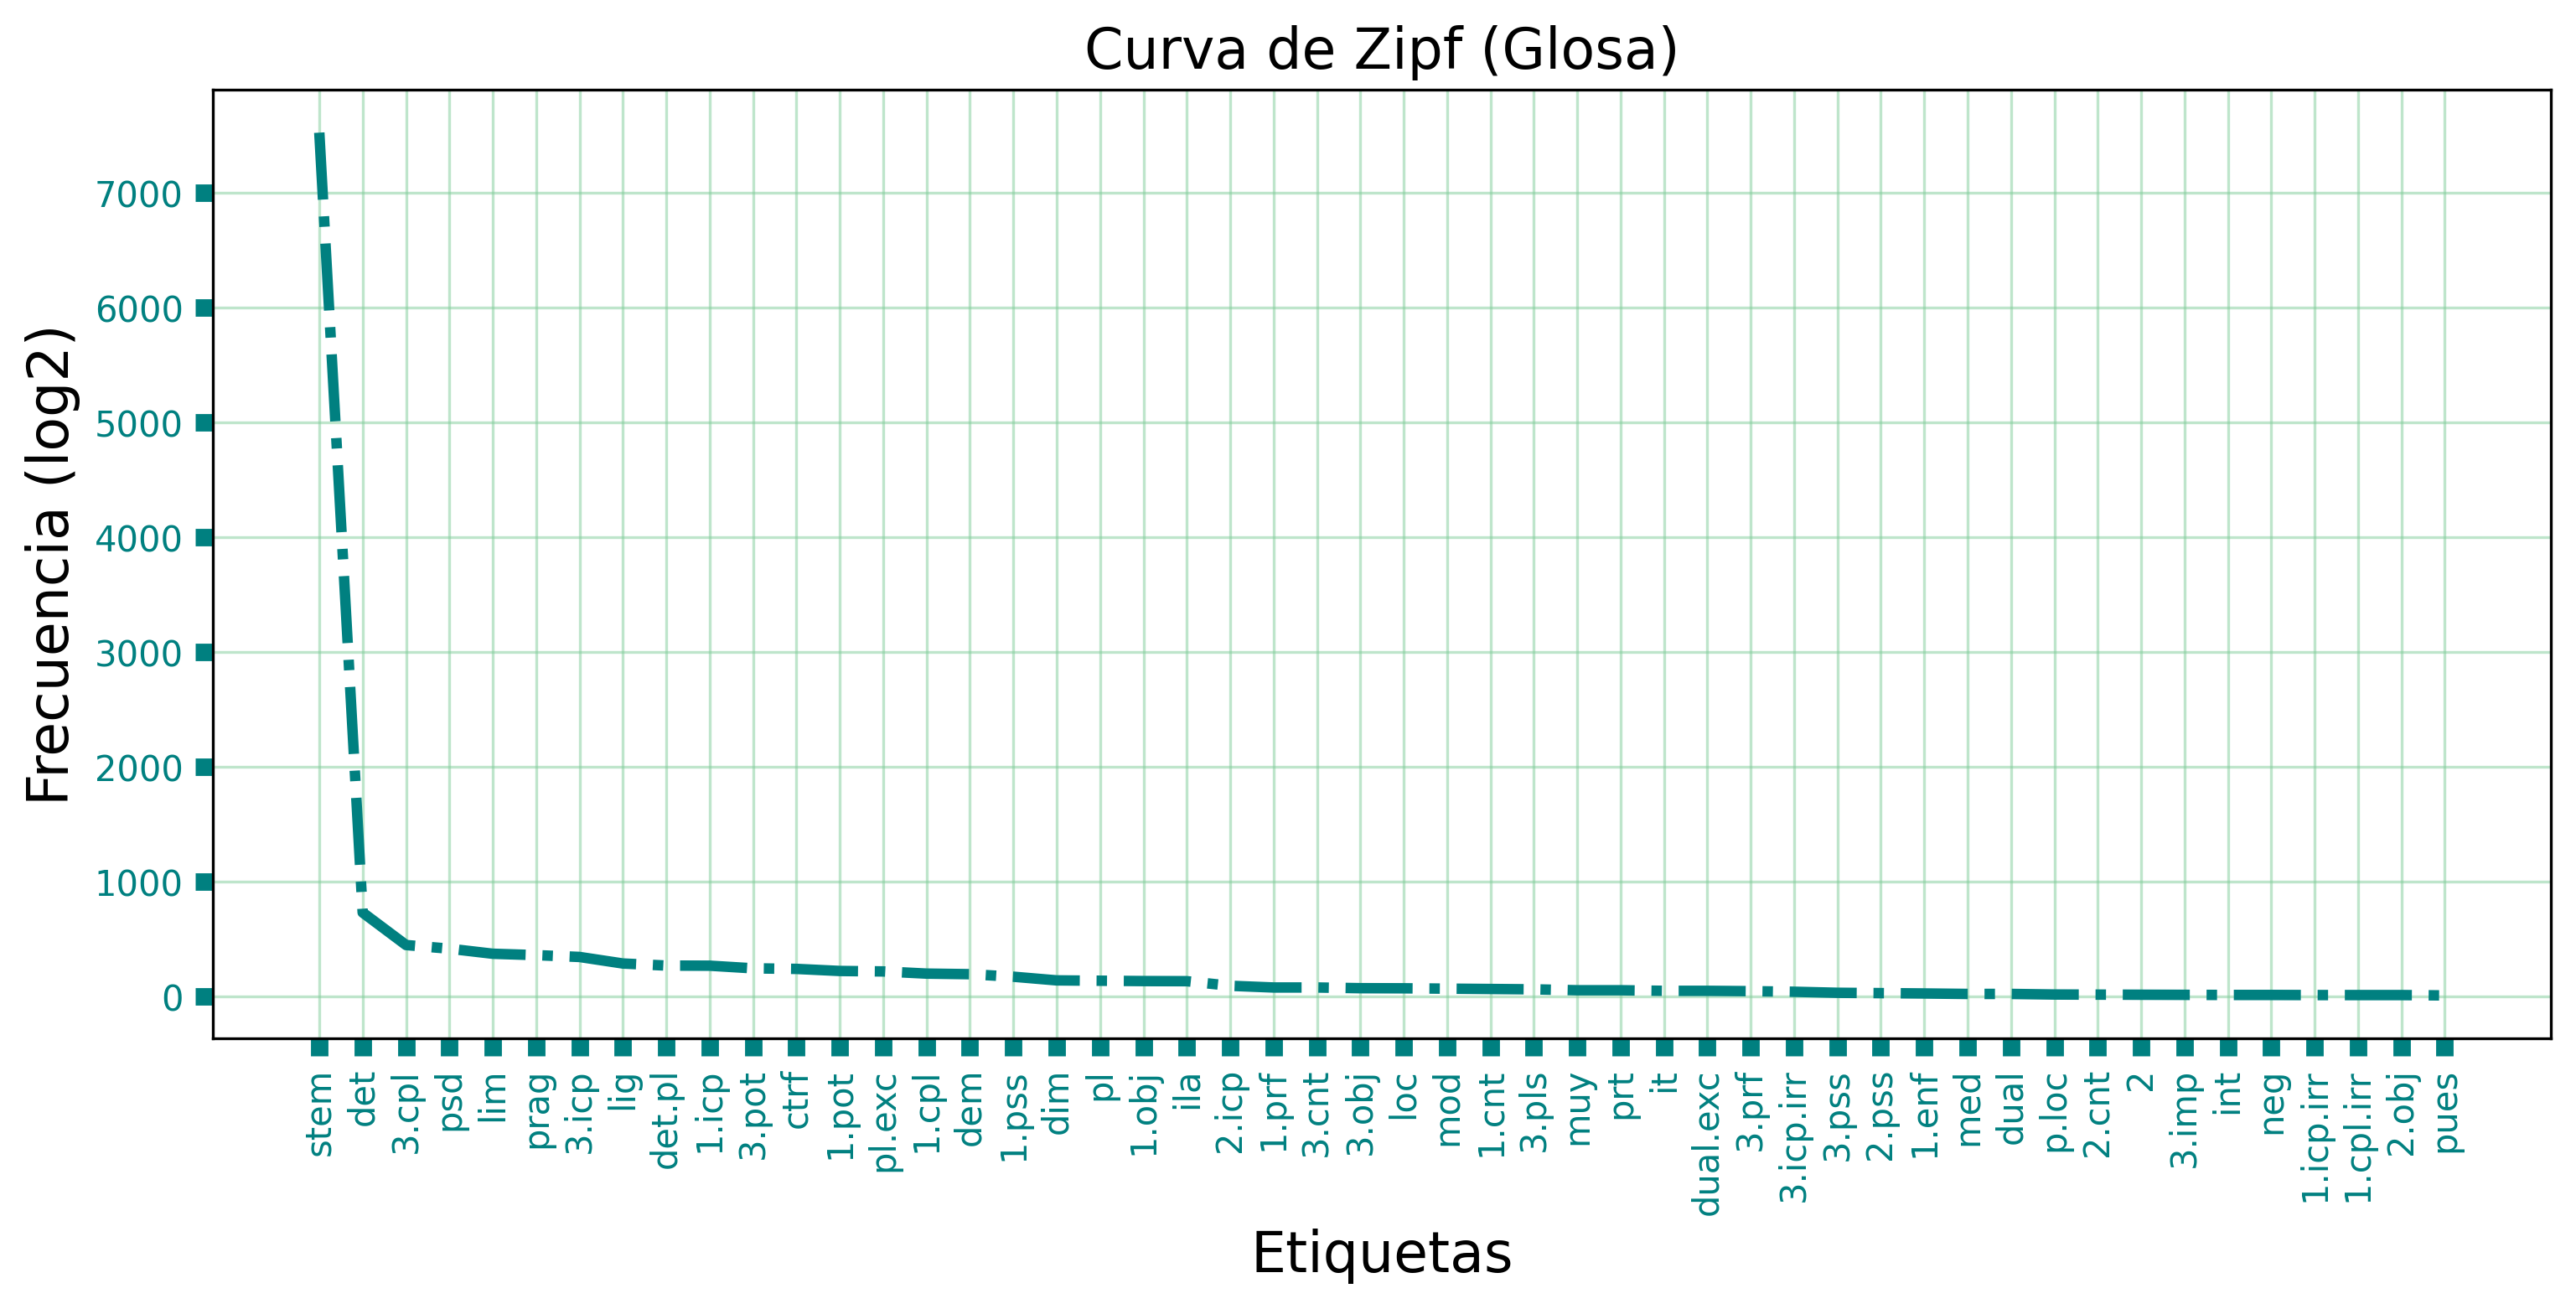
\includegraphics[width=\textwidth]{zipf_gloss}

		\caption{Distribución de glosa (primeras 50)}

	\end{figure}

	
	%5. Tipos de POS y cuantos de cada uno

	
	%Descripción general del corpus. Orientar que la arquitectura esta enfocada en

	%resolver el problema de low resources

	
	\section{Arquitectura}

	
	% Definir el método en función del marco teórico

	% Diagrama de la arquitectura

	% ¿Que es X y Y?

	% Feature functions

	% Como se decidieron

	% ¿Porque estas caracteristicas son reelevantes?

	% Que es para nosotrxs una FF

	% Experimentos quitando features functions

	% Diagram de donde se encuentran estos elementos en la arquitectura

	% Como se calculan lambdas y mu

	% Variacion de hiperparametros

	% Descripcion de que variaciones se hicieron

	% Hablar de L1 y L2 con ciertas combinaciones

	% Mostrar el base line y compararlo

	% Metodo de regularizacion y optimización

	% Mencionar que se usará un base line

	% ¿Cómo se hizo lo que se hizo?

	% Preprocesamiento del corpus

	% 

	
	Para esta tesis proponemos una arquitectura de aprendizaje estructurado débilmente supervisado utilizando el método gráfico \textit{CRF} que permitirá la predicción de secuencias que describen las unidades morfológicas (glosa) dentro de una palabra en otomí. Ya que el resultado esperado es la generación de etiquetas que, en principio, dependen unas de otras, un método basado en gráficas como los \textit{CRFs} fué el adecuado.

	
	Los \textit{CRFs} predicen las secuencias de glosa, que será la salida $Y$ dadas las observaciones $X$ (texto previamente glosado). Puntualmente, se utiliza el modelo \textbf{Markov CRF  de primer orden con \textit{features} de estado y de transición}. Adicionalmente, es utilizado el algoritmo de aprendizaje de \textbf{Limited-memory Broyden-Fletcher-Goldfarb-Shanno (L-BFGS)} como se mencionó en la sección \ref{sec:marco}.

	
	El objetivo de esta arquitectura es realizar un correcto etiquetado automático de glosa para la lengua otomí, en particular la variante del otomí de Toluca, utilizando técnicas de aprendizaje estructurado débilmente supervisado. Se definieron de aprender un conjunto de \textit{feature functions} que describen TODO el contexto y brindan información útil para la fase de entrenamiento.

	\ximena{Tener bien claro cuál es nuestra hipótesis, separarnos un poco del trabajo de lezgi}

	El \textit{pipeline} de aprendizaje semi-supervisado para la generación de glosa para

	el otomí de Toluca se describe en las secciones siguientes.

	
	% TODO: Reestructurar

	
	% Preprocesamiento

	
	% Hyperparametros

	
	% Feature functions

	\subsection{Codificación y preprocesamiento}

	
	% Obtención y preprocesamiento del corpus

	
	Se obtiene el corpus de un archivo de texto plano. Cada renglón de este archivo es una oración en otomí con glosa. Además, se tiene una etiqueta \textit{POS} por cada palabra. Las frases están estructuradas en forma de listas que contienen otras listas validas para el lenguaje \code{Python}.

	
	La glosa esta presente por cada fragmento de las posibles palabras en otomí. Ejemplificando, la frase "hi tótsogí" (\textit{No lo he dejado})\Vic{No tendría porque ir en negritas, puede ir entre '' o en cursivas. También convendría poner su traducción 'No lo he dejado'} se representa en el corpus como se muestra en el ejemplo \ref{exmp:frase_glosada}. Por último, debido a que este tipo de lenguas contienen más vocales \diego{TODO: Citar blog de elot. Incluir tabla de vocales}. Cuando se codificaban en cadenas eran separadas por el lenguaje de programación ocasionando un etiquetando de dichas marcas que por si solas no tiene sentido. Entonces, fue necesario modificar algunas letras compuestas en otomí. Las equivalencias de tales modificaciones pueden observarse en la tabla \ref{tab:letras_otomi}

	
	\begin{exmp} \label{exmp:frase_glosada}

		\code{[[['hi', 'stem'], 'neg'], [['tó', '1.prf'], ['tsogí', 'stem'], 'v']]}

	\end{exmp}

	\Vic{En este caso, el ejemplo quedaría mejor más cerca de la referencia}

	
	\begin{table}[ht]

		\centering

		\begin{tabular}{| c | c |}\hline

			\textbf{otomí} & \textbf{equivalencia} \\ \hline

			$\b{a}$ & $\alpha$ \\

			$\b{e}$ & $\epsilon$ \\

			$\b{i}$ & $\iota$ \\

			$\b{u}$ & $\mu$ \\ \hline

		\end{tabular}

		\caption{Letras en otomí modificadas}

		\label{tab:letras_otomi}

	\end{table}{}

	
	Entonces, la estructura de las listas, por renglón, tiene la estructura \code{[[[letras, glosa], [letras, glosa], ..., POS],...]}. Una vez que se obtuvo el corpus de entrenamiento se le aplicó preprocesamiento. El preprocesamiento consistió en asociar, a cada letra de cada palabra, dos elementos; la etiqueta \textit{POS} y una \textit{Bio Label} correspondiente a esa letra.

	
	Retomando el ejemplo \ref{exmp:frase_glosada} y después de aplicar el preprocesamiento el resultado sería el que se muestra en el ejemplo \ref{exmp:frase_preproc}. Cabe señalar que las \textit{Bio Labels} asignadas dependieron de la posición de la letra como se explico en la sección \ref{sec:marco}.

	
	\begin{exmp} \label{exmp:frase_preproc}

		\code{[[['h', 'neg', 'B-stem'], ['i', 'neg', 'I-stem']], [['t', 'v', 'B-1.prf'],

			['ó', 'v', 'I-1.prf'],

			['t', 'v', 'B-stem'],

			['s', 'v', 'I-stem'],

			['o', 'v', 'I-stem'],

			['g', 'v', 'I-stem'],

			['í', 'v', 'I-stem']]]}

	\end{exmp}{}

	
	Con las palabras etiquetadas a nivel de letra se obtuvo un conjunto de entrenamiento y un conjunto de pruebas. Por una parte, el conjunto de entrenamiento provee la capacidad de observar los ejemplos y así generar un modelo de aprendizaje. Por otro lado, el conjunto de pruebas nos permitió medir que tan la precisión que tuvo el modelos etiquetando frases no vistas. Es importante destacar que estos dos conjuntos estuvieron completamente separados ya que mezclar el conjunto de entrenamiento y de pruebas pudo habernos llevado a una precisión erronea y sesgada.

	
	Previo al entrenamiento se construyeron las \textit{feature functions} con el conjunto de entrenamiento. En ese sentido, por cada letra etiquetada de las palabras en otomí se tuvo una \textit{feature function} y por cada \textit{feature function} se tiene una \textit{Bio Label} asociada. La construcción de estas funciones será descrita a profundidad en la subsección \ref{subsec:feature}.

	
	% Entrenamiento

	
	Los \textit{CRFs} recibieron como entrada las \textit{feature functions}, representadas por un vector $X$ y sus respectivas \textit{Bio Labels}, representadas por un vector $y$, asociadas con cada \textit{feature function} con concordancia uno a uno respetando la posición. 

	
	\subsection{Hiperparametros}

	
	El entrenamiento consistió en la búsqueda de un modelo que maximiza el logaritmo de verosimilitud con el método de aprendizaje \textit{L-BFGS}. Es necesario entonces definir los parámetros del algoritmo de maximización. Utilizamos \textit{Elastic Net} con los valores de regularización, necesarios para evitar problemas como el \textit{overfitting}, L1 + L2 y el máximo de iteraciones. Ya definidos los hiperparametros se ejecutó la fase de entrenamiento.

	
	% Testing

	Una vez terminada la fase de entrenamiento y construido el modelo de aprendizaje se puso a prueba con el conjunto destinado a este propósito y que fue previamente obtenido. Similar a la fase de entrenamiento las entradas fueron las \textit{feature functions} y sus respectivas \textit{Bio Labels}. Utilizando el modelo de aprendizaje se etiquetó cada letra con base en la información de las \textit{feature functions}. Las etiquetas generadas fueron comparadas con las reales y se obtuvo la exactitud del modelo. 

	
	% Pasar a resultados

	Consideramos exitosa la predicción si se logra maximizar la correcta clasificación de las secuencias de salida. Para determinar si la predicción fue exitosa se utilizaron técnicas típicas de \textit{ML} como \textit{K-folds} que consiste en tomar \textit{K} fragmentos de los datos de entrada y utilizarlos para probar el modelo. Además de reportar la precisión se obtuvo el \textit{recall} y \textit{F-score}.

	
	\subsection{Feature functions} \label{subsec:feature}

	
	La extracción de estas características es importante porque capturar fenómenos lingüísticos necesarios para que la estructura de la lengua se pueda plasmar en el modelo de aprendizaje. Estas características están capturando, entres otras cosas, el contexto de la palabra y es importante para predecir la morfología. Para construir las \textit{feature functions} se necesita el corpus glosado y etiquetado a nivel de letra. Se extrajeron las siguientes características para cada letra en el corpus:

	
	
	% TODO> Explicar mas cada una

	\begin{itemize}

		\item \textsf{bias}: Esta característica captura la proporción de una etiqueta dada en el conjunto de entrenamiento. Ayuda a tomar en cuenta que algunas etiquetas son poco usuales y otras muy usuales. % TODO> Hablar del bias en general

		\item \textsf{letterLowercase}: Toma la letra y la convierte a minúsculas. Es importante para la creación del modelo tener en cuenta la letra que se esta viendo en un momento determinado para las predicciones posteriores.

		\item \textsf{prevpostag}: Toma la etiqueta POS previa (Si existe)

		\item \textsf{nxtpostag}: Toma la etiqueta POS siguiente (Si existe)

		\begin{itemize}

			\item Es conveniente y muy útil tomar en cuenta las etiquetas \textit{POS} ya que brindan información gramatical de la palabra que se observa en ese momento. Tal información se basa en la morfología y algunas veces en la sintaxis de la lengua.

		\end{itemize}

		\item \textsf{BOS}: Indica el inicio de la frase

		\item \textsf{EOS}: Indica el fin de la frase

		\item \textsf{BOW}: Indica el inicio de la palabra

		\item \textsf{EOW}: Indica el final de la palabra

		\begin{itemize}

			\item Indicar el inicio y fin de frase y palabras otorga la capacidad de ver que tipo de palabras se está viendo en ese momento. Por ejemplo, una palabra que esté justo al inicio de una oración en general será un ..., mientras la palabra al final de una oración probablemente será un ... \diego{Duda de que estructuras son comúnes en otomí}  

		\end{itemize}

		\item \textsf{letterposition}: Indica la posición de la letra en la palabra

		\item \textsf{prev4letters}: Toma las cuatro letras previas (Si existen)

		\item \textsf{prev3letters}: Toma las tres letras previas (Si existen)

		\item \textsf{prev2letters}: Toma las dos letras previas (Si existen)

		\item \textsf{prevletter}: Toma la letra previa (Si existe)

		\item \textsf{nxtletter}: Toma la siguiente letra (Si existe)

		\item \textsf{nxt2letters}: Toma las siguientes dos letra (Si existen)

		\item \textsf{nxt3letters}: Toma las siguientes tres letra (Si existen)

		\item \textsf{nxt4letters}: Toma las siguientes cuatro letra (Si existen)

		\begin{itemize}

			\item La recuperación del varias ventanas contexto son convenientes para del otomí ya que se trata de una lengua aglutinante dónde, en general, las palabras son largas. En particular, la longitud promedio de las palabras en el corpus es de 4.89. Esta característica da la pauta para que la observación del contexto en un determinado momento sea relevante para la construcción del modelo.

		\end{itemize}

	\end{itemize}

	
	Las características mencionadas son información relevante para poder construir un modelo más preciso dadas las estructuras de la lengua. Dichas características pueden o no estar presentes dependiendo de la letra que se esté viendo en ese momento. Por ejemplo, si es la primer letra de una palabra la que se observa no estarán presentes las características \textsf{prevletter}, \textsf{prev2letters} o \textsf{EOW} por mencionar algunas. Características como \textsf{letterLowercase} o \textsf{bias} siempre estuvieron presentes.

	
	\subsubsection{Hardware utilizado}

	
	En la fase de experimentación fue utilizado el paquete \textsf{python-crfsuite} que es un \textit{binding} de la implementación de TODO:CITA para CRFs para lenguaje de programación \textit{Python} en su versión \textit{3.7}. La fase de experimentación corrió en una maquina con un procesador \textsf{Intel i7-7700HQ @ 3.800GHz} con \textsf{16 GB} de memoria principal. En promedio una corrida de entrenamiento y evaluación \textit{K-folds} con \textit{k=10} tomó 52 minutos.

	
	% TODO: Resumen al final (pasos de todo lo que se hizo)

	
	\chapter{Resultados}

	
	% Solo reportar

	
	% Mostrar la comparación a profundidad del baseline con todos los experimentos

	% Demostrar que lo que propusimos fue mejor

	% Cualitativos y cuantitativos

	% Hablar del Baseline y como mejoró con mas features

	% explicar como ayudo la información de las Feature functions

	% Definir como plantear la historia: 

	% De lo mas básico (baseline) y ver como lo mejoramos con las feature functions

	% El conocimiento lingüístico ayuda a mejorar

	
	\section{Corpus de evaluación}

	
	\section{Evaluación}

	
	% Aquí se habla del K fold y de como se introdujo el corpus retador.

	
	\section{Análisis de resultados}

	
	% Cual salio mejor

	% cual salio pero

	% logramos pasar el base line?

	% que features fueron determiantes?

	
	
	\chapter{Conclusiones}

	
	\bibliography{tesis}

	
\end{document}